% vim:spelllang=en_us:spell
% Author: Marek Filip 2022

\chapter{Introduction}

When we look at cryptocurrencies, there is a very lucrative market. That is why people have always found new ways to make money from trading cryptocurrencies. There are many trading strategies for cryptocurrencies available, but no such strategy survives both rising (bull) and falling (bear) market. That is why there is a need for adaptive strategies that can prosper through both of them.

I will explore the idea of the adaptive trading strategies for cryptocurrencies in this thesis. Firstly we need to find a way how to predict if the market will go up or down. Then we need to apply sufficient trading strategies regarding the percentage probability of market going up or down. That is the basic idea.

To get to this point I will explore the current trading strategies that are used for trading cryptocurrencies. Analyze current simulation tools available today and analyze the historic trading data to find some patterns. Looking at current state of adaptive strategies for cryptocurrencies is also necessary.

\subsection*{Organization}

The rest of this work is divided into several chapters.

Firstly, there is the chapter \ref{background}, which gives the reader a sufficient theoretical background that is required to understand the later chapters of the thesis. In the chapter \ref{trading-stategies} I look at the existing trading strategies and analyze their effectiveness. In the chapter \ref{simulation-tools} several existing simulation tools are explored and compared. I also analyze the backlog of cryptocurrency trading data provided by the supervisor and summarize the important events.


\chapter{Background}
\label{background}

There are some prerequisites that the reader must be familiarized with in order to understand the thesis. The basic knowledge of what a cryptocurrency is must be explained. As well as clear understanding of some terms that are regularly used in the thesis.

\subsection*{List of terms generally used in the thesis and among crypto investors}
\begin{itemize}
    \item Best strategy = A strategy that yields the most money -- has the best profit.
    \item Bear market = A market in which prices are falling, encouraging selling.
    \item Bull market = A market in which prices are rising, encouraging buying.
    \item FOMO = Fear of missing out.
    \item FUD = Fear, uncertainty, doubt.
    \item Fiat currency = Government-issued money.
    \item ROI = Return of investment.
    \item spread = Difference between buy and sell value of an asset.
\end{itemize}

\section{What is a cryptocurrency?}
\emph{Cryptocurrency} is a digital currency that is secured by cryptography \cite{investopedia-cryptocurrency}. There are algorithms in place that make it nearly impossible to counterfeit or double-spend the currency. Cryptocurrencies are based on a decentralized networks based on the blockchain (see \ref{blockchain}) technology. Because of this the cryptocurrencies are not issued by any central authority (unlike conventional currency). This makes them theoretically immune to government interference or manipulation.

\subsection*{Types of Cryptocurrency}
\emph{Bitcoin} is the original and to this day the most popular and valuable cryptocurrency. It was invented by an anonymous person called \emph{Satoshi Nakamoto} in 2008 via a white paper \cite{satoshi}. As of 12th January 2022, there are over 18.9 million bitcoins in circulation with a total market capitalization of around \$810 million \cite{coinmarketcap}, making it roughly 40\% of the total cryptocurrency market.

Each new cryptocurrency claims to have different function and specification. New cryptocurrencies are created daily. Most are not lucrative to investors at all while others surprise the market with their new innovations. For example, Ethereum's \emph{ether} markets itself as a gas for their underlying smart contract\footnote{https://www.investopedia.com/terms/s/smart-contracts.asp} platform. Another example is Ripple's \emph{XRP} which aims to facilitate international bank transfers. New cryptocurrencies started to rise due to bitcoin's many unsuitable aspects.

\label{stablecoins-ref}
A \emph{stablecoin} is another important type of cryptocurrency. It aims to offer price stability and is backed by a reverse asset\footnote{https://www.investopedia.com/terms/r/reserve-assets.asp} like the US dollar. They attempt to offer the best of both worlds---the instant processing and security of privacy payments of cryptocurrencies, and the non-volatile character of fiat currencies \cite{investopedia-stablecoin}.

\subsection*{What is FIAT money?}
Fiat money or currency is money that is issued by the government and is not backed by any gold or other physical commodity. Its value is derived between the relationship of supply and demand and the stability of the government that issued it \cite{investopedia-fiat}. It represents today's currencies of the world. Many crypto enthusiasts believe that cryptocurrencies will replace fiat currencies in the future.

\subsection*{Blockchain}
\label{blockchain}
Blockchain or a distributed ledger\footnote{https://www.investopedia.com/terms/d/distributed-ledger-technology-dlt.asp} is a digital database that is shared and synchronized across a distributed network consisting of very large number of computers \cite{investopedia-blockchain}. Distributed networks eliminate the need for central authority to keep a check against manipulation. You can see the blockchain's basic structure in Figure \ref{blockchain-figure}.

\begin{figure}[ht]
    \centering
    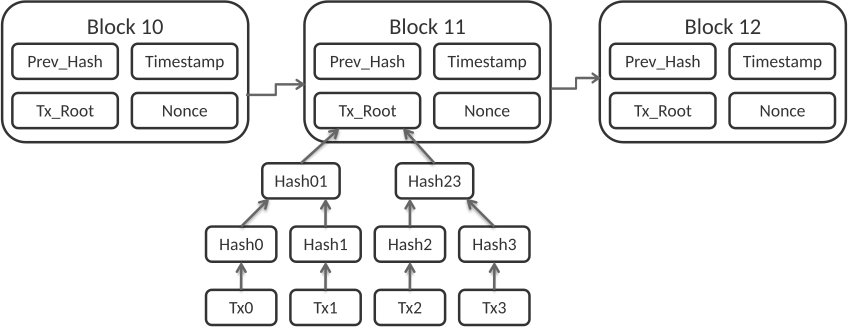
\includegraphics[width=\columnwidth]{figures/Bitcoin_Block_Data.png}
    \caption{Blockchain structure, attribution: Wikimedia}
    \label{blockchain-figure}
\end{figure}

\section{What are bear and bull markets?}
While you may know that the bear and bull markets stand for falling and rising markets, there is more to these terms that must be explained. The origin of the terms themselves is believed to be tied to the way the two animals attack their opponents. A bull thrusts its horns up, while a bear swipes its pawns downwards \cite{investopedia-bull-market}.
Herd behavior is important to consider when talking about the terms.

\subsection*{Bear Market}
As growth prospects wane and expectations are unmet, prices decline \cite{investopedia-bear-market}. Bear markets are viewed as pessimistic with investors scared to open new positions. But to talk about bear or bull market we usually ascribe longer time periods than the usual and always present volatility of the crypto market. For example when China declared all of the cryptocurrency transactions illegal \cite{china-ban}, a fall of crypto markets quickly ensued.

A bearish investor or bear is then a type of investor that believes that a specific coin is likely to decline in the future \cite{investopedia-bull}.

\subsection*{Bull Market}
Bull markets are characterized by optimism, investor confidence and expectations in strong results that will continue for a long period of time \cite{investopedia-bull-market}. FOMO\footnote{Fear of missing out.} is present among investors. Both bull and bear markets are hard to define, bull market is usually specified to occur when prices rise by $20\%$ after a previous $20\%$ drop and before another $20\%$ drop---these values are defined for stock markets only, so the margins should be higher for the volatile cryptocurrency market.

A bullish investor or bull is a type of investor that believes that a specific coin is likely to rise \cite{investopedia-bull}.

\chapter{Trading Strategies for Cryptocurrencies}
\label{trading-stategies}

There are various trading strategies available regarding cryptocurrencies.
In this chapter we will go through those that are considered the most well-known and consider
their ups and downs.

\section{HODL}

This is the strategy that is one of the most prominent in the cryptocurrency market, especially by beginners to trading.
It is jokingly derived from misspelling of the word "hold". The original post by the user GameKyuubi \cite{hodl-post} containing the misspelling was originally posted on 18th December 2013, from which it quickly spread on.

HODL or "hodl on for dear life" has become a slogan among crypto enthusiasts, representing long-term approach to cryptocurrency trading. It implies that the novice traders are not successful in timing the market so they should simply hold the coin until the prices significantly rises.

Cryptocurrency maximalists keep HODLing, because they believe that cryprocurrencies will eventually replace the government-issued fiat currencies as the basis of all economic structures \cite{investopedia-hodl}.

\section{Rebalance}
Rebalancing is the process of realigning the weightings of portfolio of assets---in our case cryptocurrencies. It involves periodically buying or selling the assets in portfolio so that the original level of asset allocation is maintained\cite{investopedia-rebalancing}.

For example if we set portfolio allocation 50/50 to BTC and ETH coins. And the BTC coin rised by 20 \% so that the new ratio would be 70/30, we would sell the 20 \% of the BTC and for the value we got we would buy additional ETH coins, so that the ratio is again 50/50.

Rebalancing gives investors the opportunity to sell high and buy low. It takes gains from high-performing investments and reinvests them in areas that have not yet grown that much.

One study \cite{portfolio-rebalancing}, conducted by the Shrimpy Team, has found that rebalancing beats hodl by a median of $64\%$. The analysis was performed with 1-year period real trading data.

There many types of rebalancing strategies. We will look at some of them now.

\subsection*{Periodic Rebalancing}
This is the simplest rebalancing to use. The rebalance happens after a fixed amount of time. For cryptocurrencies it makes sense to set shorter time due to rapid price fluctuations, something like 1 day.

\subsection*{Threshold Rebalancing}
A more interesting approach is threshold rebalancing where we set some threshold deviation. When an allocation deviates by that set threshold from the original allocation, a rebalance happens, setting all the allocations to their original values \cite{portfolio-rebalancing}.

Let's say we once again have 50/50 BTC/ETH allocations. Let's set the threshold deviation to $20\%$. If the price of BTC or ETH reaches over 60\% or under 40\%, a rebalance takes place. 20\% out of 50\% is 10\%, that is why the rebalance happens at those points. When both coins grow or decline in the same rate, no rebalance happens.

\subsection*{Assumptions}
One study around rebalancing has been already mentioned, let's look into some of them in more detail now. The studies \cite{portfolio-diversity} and \cite{diversify-perform-better} conducted by the Shrimpy organization have found some interesting results. Both of the studies took into account only periodic rebalancing. They have found that the shorter the time period for rebalance, the better the results, maximizing them at 1 hour period. The other interesting discovery was that if the portfolio had more assets in it---was more diversified---the better were the results. The diversification really took advantage of the sell high buy low formula.

Another study \cite{rebalancing-strategy} confirmed that a portfolio with a larger number of assets performs better. Some other interesting facts have been observed during the simulations that improve the performance of the portfolio:
\begin{itemize}
    \item Equal weightings of the allocated assets.
    \item Assets that are uncorrelated or negatively correlated with each other. That means if one rises, the other should go down.
    \item Assets that have similar rates of return, though volatility also improves the performance.
\end{itemize}

\section{Dollar Cost Averaging}
Dollar Cost Averaging (DCA) is a strategy often recommended to the beginner investors. The investor makes periodic purchases of the asset in an effort to reduce the volatility of the market. This removes much of the detailed work needed to time the market in order to make purchases at the best price.

Through studies \cite{DCA-study} it seems that the advantage of DCA lies more in the reduced psychological effort in order to time the market than in the actual results. Single buy-and-hold strategy seems to outperform DCA in more cases.

Sometimes DCA is used as a mean to invest into trusted assets on weekly/monthly basis---when employees get money. It is also used in some employment plans\footnote{For example the American 401(k) plan} across the world.

\section{Day Trading}
Day trading are the investors that buy and sell the same asset over the span of one day. They might even buy and sell the assets multiple times. They mostly use technical analysis of the market to achieve this goal. It is not recommended for beginner investors to choose this type of trading as it is much more risky than strategies described before.

\section{Range Trading}
Asset move in certain ranges, as you can see in Figure \ref{trading-range-figure}. Range trading assumes that and tries to take guesses where are the limits using candlestick charts and support and resistance levels. Investors want to buy when prices reach the support level and sell when they reach the resistance level \cite{5types-of-daytrading}. The support and resistance levels can be seen in Figure \ref{sup-and-res-levels}.

\begin{figure}[ht]
    \centering
    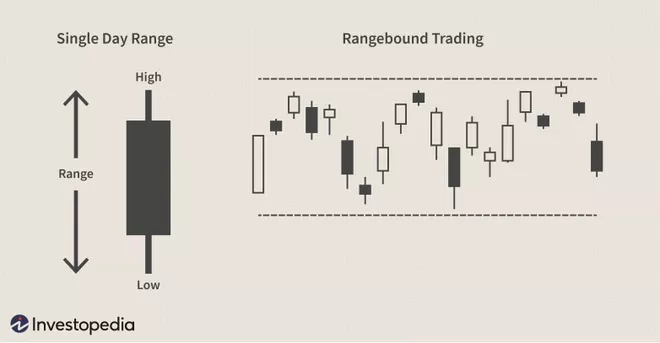
\includegraphics[width=\columnwidth]{figures/trading-range.png}
    \caption{Trading range visualization, attribution: Investopedia \cite{investopedia:trading-range}}
    \label{trading-range-figure}
\end{figure}

\begin{figure}[ht]
    \centering
    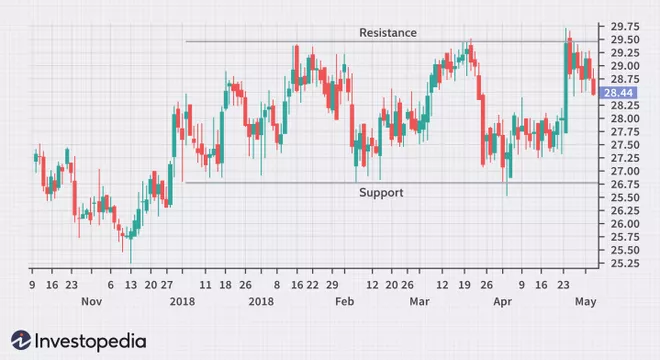
\includegraphics[width=\columnwidth]{figures/dotdash-final-trading-range.png}
    \caption{Support and resistance levels, attribution: Investopedia \cite{investopedia:trading-range}}
    \label{sup-and-res-levels}
\end{figure}

\section{Scalping}
In scalping you try to profit from very small price movements over short periods, you might exit a trade seconds after entering it. It is best to use automated bots to increase the buying frequency. Scalpers take advantage of increased trading volume to profit. They want to exit before any news or short-term fluctuation changes the market's view of the coin \cite{best-crypto-daytrading}.

It is needed to have a large bankroll to use this strategy effectively. Since the return of investment is really low, the amount gain must be significant enough. It also needs to cover trading fees.

In Figure \ref{scalping-figure} it can be seen how scalping can take quick and short advantages of the market.

\begin{figure}[ht]
    \label{scalping-figure}
    \centering
    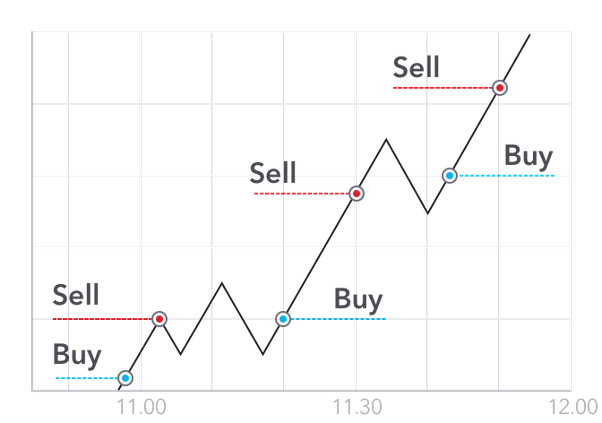
\includegraphics[width=\columnwidth]{figures/scalping.png}
    \caption{Scalping visualization, attribution: Quora \cite{best-crypto-daytrading}}
\end{figure}

\section{Automated Trading Systems or Bots}
\label{bots}
Automated trading systems---also referred as algorithmic trading---allow investors to set specific rules for enter and exit of a trade that can be automatically executed via computer program. Some platforms claim that 70\% to 80\% of trading done comes from the automated systems \cite{investopedia-bot-trading}.

One of the advantages is that the automated trading systems take emotions out of the trading---they only work on a specific criteria. The automated trading systems need to use software or APIs available from the broker. The outcome made in this thesis is expected to be used by some automated trading system.

Automated trading systems are one of the only options to use when considering strategies like scalping due to the ease of getting in and out of a trade in seconds without room for failure. The software also allows backtesting the chosen strategy on historical data from which it can be seen how well it does perform.

\section{Arbitrage}
Arbitrage involves buying cryptocurrency in one market and selling it for higher price in another one. Since the cryptocurrency market is usually unregulated, anyone can make an exchange. This can lead to major differences in the spread of the asset.

There are two types of arbitrage when it comes to cryptocurrencies. The first one focuses on finding prices mismatches across different trading pairs on a single exchange. The other is the one that was already described---locating significant price differences on multiple exchanges. Both types take advantage of an automated trading system that monitors the exchanges and looks for price differences. In Figure \ref{arbitrage-figure} you can see how the first type can be profitable.

Regarding the second type of exchange. In January a legendary \emph{kimchi premium}\footnote{https://www.investopedia.com/terms/k/kimchi-premium.asp} happened. Bitcoin traded almost 40\% higher on the Korean exchanges that the US exchanges. This lead to arbitrage investors taking advantage of this fact, buying bitcoin on US exchanges and selling it on the Korean ones for profit \cite{hodlbot:day-trading-cryptocurrency}.

\begin{figure}[ht]
    \centering
    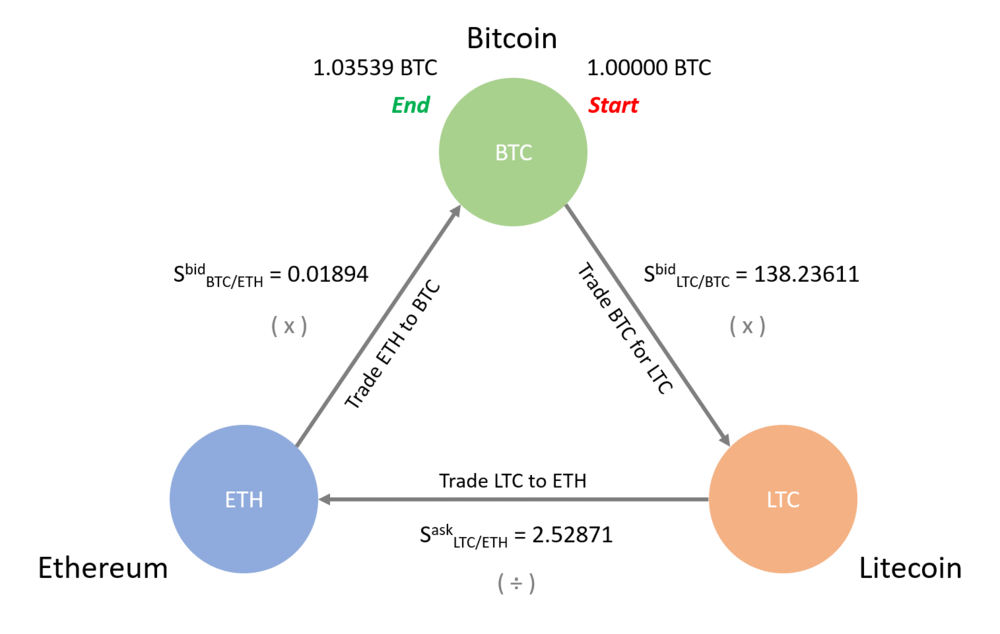
\includegraphics[width=\columnwidth]{figures/arbitrage.png}
    \caption{Arbitrage execution via multiple trading pairs, attribution: HodlBot \cite{hodlbot:day-trading-cryptocurrency}}
    \label{arbitrage-figure}
\end{figure}

\section{Stablecoin Trading}

When talking about different trading strategies, the focus is usual on the method of the trategy, not the asset themselves. But when it comes to specific thing like stable coints, there is an opportunity to handle them in such a way to generate profits for us.
The term stablecoin has already been explained in \ref{stablecoins-ref}. It is a coin which has its value pegged to some external reference.

For example it was found in \cite{make-money-stablecoins} that a de-pegging of stablecoins happens periodically often as a result of temporary shock to the crypto system. During those events profit can be made when trading pegged and de-pegged stablecoins between each other. The author chose DAI and USDC pair for their experiments. It was shown that between August 2019 and March 2020 the spread between DAI and USDC has been fluctuating between 2 to 3\%. Advantage could be taken of this fact---selling DAI for USDC when the price is high and buy it back for USDC when the price returns to the peg.

One thing to remember is to only trade when the spread is sufficient so that the trading fees won't make the profit diminish.

\chapter{Existing Simulation Tools for Testing Trading Strategies}
\label{simulation-tools}

In this chapter different simulation tools, their application, usefulness and differences, are discussed. We must distinguish few types of simulation tools when talking about them. When a novice investors first sets foot in the cryptocurrency market, they might be startled by the complexity of the market. They want to learn, but maybe they do not want to lose all their money in the process. That is the perfect opportunity for a manual simulated tool. Investors can invest fake virtual money while all of the market's trading data is accurate and up to date.

\section*{Types of cryptocurrency simulators}

\begin{enumerate}
    \item Cryptocurrency market games
    \item Virtual trading simulators
    \item Backtesting simulation tools
\end{enumerate}

\emph{Cryptocurrency market games} are games that have less emphasis on the trading skills and more on the entertainment of trading. They are mostly fun way to compete with your friends or strangers. The player that creates the strongest portfolio is considered the best. The winner is then the player with the best investments at the end of the specific game. \cite{top-stocks-crypto-trading-simulators}.

\emph{Virtual trading simulators} are simulators where users can closely track the real market and actively trade cryptocurrencies for virtual profit \cite{top-stocks-crypto-trading-simulators}. The main goal is to use the simulated experience for building and improving the real life trading skills of the user. You can test-drive and backtest your strategy here.

\emph{Backtesting simulation tools} are similar to the virtual trading simulators in a way, that it aims to make its users better at trading. While the conventional trading simulators only work in real time, there are simulation tools where its users can input chosen strategy and see it run across multiple years of historical data and see how it performed in seconds. This is the type of simulation tools that will be used in this thesis. It basically uses backtesting for the cryptocurrency strategy's validation.

\section{What is Backtesting?}
The section was inspired by this source \cite{backtesting-crypto-trading-strategies}.

Backtesting means applying a trading strategy or some analytical method on a historical data and analyzing the performance of the current strategy or method. If the strategy shows promise, the trader may use it in a live environment on an exchange. Backtesting does not guarantee future results, but can be a good indicator and filter the effective strategies from the ineffective ones. Backtesting can also detect recurring patterns and exploit those patterns for profits.

\subsection*{Discretionary Backtesting}
Discretionary backtesting is a manual form of backtesting. The trader manually places buy and sell order with each signal they receive. They trader may decide to conduct the testing using software such as TradingView\footnote{https://www.tradingview.com/}.

The trader will set a strategy in place, then he will press the replay button (shown in Figure \ref{tradingview-figure}) and select period of history to test on. The trader will then make discretionary decisions to buy or sell based on the signals.

Manual testing is a great way to control trader's emotions since they may feel the same emotions as in live environment. The disadvantage is that it is quite time-consuming. Trader may run a test for hours only to find out it was not a good strategy (though this result is also valuable). Secondly the amount of data the trader can test the strategy on is limited.

\begin{figure}[ht]
    \centering
    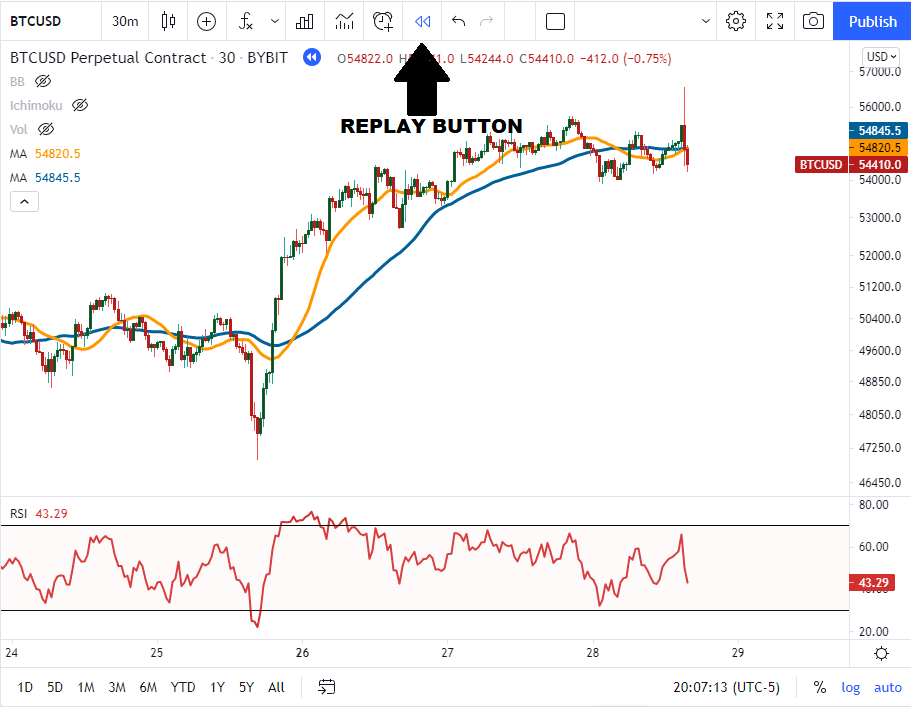
\includegraphics[width=\columnwidth]{figures/tradingview-replay.png}
    \caption{TradingView replay functionality, attribution: TradingView \cite{backtesting-crypto-trading-strategies}}
    \label{tradingview-figure}
\end{figure}

\subsection*{Systems Backtesting}
Systems backtesting offers the trader the true power of technology. Systems traders will have a strategy coded and the program will test the strategy against the historical data while generated statistics of the achieved results in manner of seconds. This will show the trader useful statistics about the strategy and help him decide if it is robust and well-performing enough to use in a live environment.

The challenge of systems backtesting is to have sufficient technical knowledge on how to create such algorithmic strategies. And also the analytical knowledge to determine if the strategy performed well or not.

\subsection*{Automated Backtesting}
Automated or \emph{algorithmic} trading refers to traders who use a computer program to execute a trade, as explained in \ref{bots}. Backtesting of strategies can also be automated this way and is usually just another name for systems backtesting. We automate the results to arrive at helpful statistic to help us determine effective strategies. It is conducted using a programming language.

\subsection*{Simulated Backtesting}
Simulated backtesting simply means running a test over a historical data that simulates the real market environment. In this example the system is market environment and the model is the simulated environment.


\section{Data requirements for backtesting}
Systems traders will want to simulate the real-world data as closely as possible. Trading costs such as commissions, exchange spreads and slippages can chew away the expected returns. This costs can throw off the backtest results if ignored.

Both \emph{candlestick} and \emph{order book data} are used in backtests, though order book data is usually more reliable.

\subsection*{OHLCV Candlestick Data}
\label{ohlcv-candlestick-data}
OHLCV stands for Open-High-Low-Close-Volume, you can see how they can be represented in Figure \ref{OHLCV-figure}. The candlestick data itself is visualized in Figure \ref{candlestick-figure}. It is essentially a spreadsheet of price data of the chart time frame. If you pull the candlestick data for the daily chart of Bitcoin, you will receive each day's open, high, low and close price data. If you request 1-minute data, the spreadsheet will include each minute's open, high, low and close price for Bitcoin on that particular day.

OHLCV abbreviations explained \cite{kaiko-ohlcv}:
\begin{itemize}
    \item Open: Price at which the asset started at the time interval.
    \item High: Highest price reached during the time interval.
    \item Low: Lowest price reached during the time interval.
    \item Close: Price at which the asset ended after the time interval.
    \item Volume: Quantity of asset bought or sold, displayed in base currency.
\end{itemize}

\begin{figure}
    \centering
    \begin{subfigure}[t]{0.45\textwidth}
        \centering
        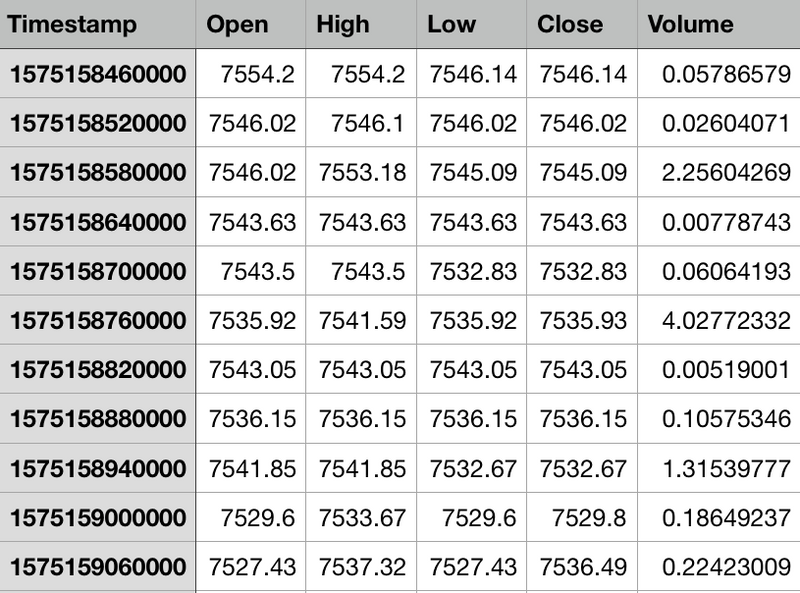
\includegraphics[width=\textwidth]{figures/OHLCV-data.png}
        \caption{How can OHLCV data look like, attribution: Kaiko \cite{kaiko-ohlcv}}
        \label{OHLCV-figure}
    \end{subfigure}
    \hfill
    \begin{subfigure}[t]{0.45\textwidth}
        \centering
        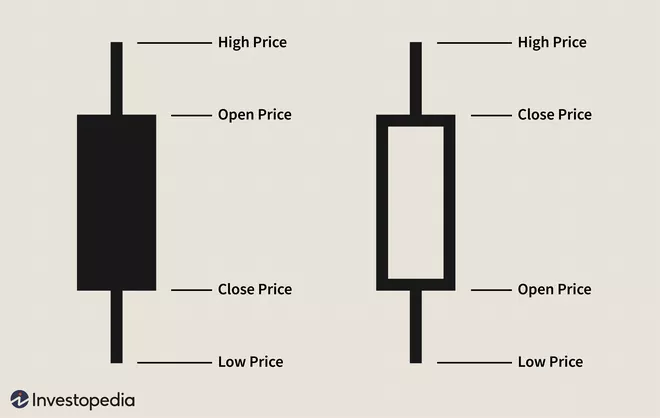
\includegraphics[width=\textwidth]{figures/candlestick-data.png}
        \caption{Candlestick explained, attribution: Investopedia \cite{investopedia:candlestick-charts}}
        \label{candlestick-figure}
    \end{subfigure}
    \caption{OHLCV Candlestick Data}
\end{figure}

There are several imperfection to the OHLCV candlestick data. Firstly, there is no information which prices have been traded for which volume. Additionally, if a trader has a large account, there might not be enough cryptocurrency available to trade without moving the market price---negatively impacting the backtest results. Traders typically use candlestick data because it is easiest to acquire.

\subsection*{Order Book Data}
An order book is one of the best data sources and resolves some challenges of the candlestick data. It includes snapshots of the market, including the market's price, volume and depth. With this type of data traders have a better representation of what orders are available at any given time.

It allows testers to simulate bid-ask spread, slippage and liquidity when testing a particular strategy. All of these unavailable to testers using candlestick data. The challenge with order book data is that it is hard to come by. There is tremendous amount of data with order book snapshots so the exchanges choose not to hold the data, as it would be too expensive to store. Therefore usually the developers needs to collect and store the data from the exchange themselves or access the snapshots through a third-party service.

\section{Performance Analysis}
\label{performance-analysis}
This section was again inspired by the \cite{backtesting-crypto-trading-strategies} source.

Performance of the given trading system or strategy is commonly gauged against parameters such as profit and loss (P\&L), success ratio, and Sharpe ratio.

\subsection*{Profit and Loss -- P\&L}
Once the desired strategy has been created and backtest executed, the big number traders will be interested in is the profit. The backtest should spit out P\&L analysis by trade and day. That way an equity curve can be created, showing what the balance would have been if it were traded live. Equity curve is just a time series chart showing what the value of the account would have been after each passed day.

P\&L analysis also generates the size of the average winning and the size of the average losing trade. Taking the ratio of those two averages you get a useful average risk-to-reward ratio. For example if the average winning trade is \$100 and the average losing trade is \$50 you get a $1:2$ risk-to-reward ratio.

\subsection{Success Ratio}
The success ratio is the win ratio of the strategy. Let's say a strategy makes 100 trades. If 72 of those trades are profitable, it has 72\% success (or win) ratio. By itself the ratio does not tell much and might be misleading. It is best coupled with the average winner and the average losing trade ratios mentioned in P\&L.

For example, a success ratio of 58\% and 1:2 risk-to-reward ratio indicates a very good strategy.

\subsection{Sharpe Ratio}
This subsection was sourced from \cite{investopedia:sharpe-ratio}

The Sharpe ratio, developed by \emph{William F. Sharpe}, is used to understand the return of an investment (ROI) compared to its risk. The ratio is the average return earned in excess of the risk-free rate per unit of volatility or total risk.

$$Sharpe\ ratio = \frac{R_p - R_f}{\sigma _p}$$
where:
\begin{itemize}
    \item $R_p$ = return of portfolio
    \item $R_p$ = risk-free rate
    \item $R_p$ = standard deviation of the portfolio's excess return
\end{itemize}

Generally, the greater the value of the Sharpe ratio, the more attractive the risk-adjusted return. The yield for the US Treasury bound is often used as the risk-free ratio. One of the limitation of the Sharpe ratio is that it assumes that the returns are normally distributed, which is simply not true.

\section{Popular simulation tools}
Some popular and easily available simulation tools are Holderlab\footnote{https://holderlab.io/}, Zenbot\footnote{https://github.com/DeviaVir/zenbot}, Gekko\footnote{https://gekko.wizb.it/}, Altrady\footnote{https://www.altrady.com/}, and Binance's Python backtesting\footnote{https://www.binance.com/}.

\section{What type of cryptocurrency simulation tool should we use?}
When looking at the explored simulation tools it is clear that an automated backtesting program will be used to test the proposed adaptive trading strategy. I will use the OHLCV candlestick data provided by the supervisor and look for order book data if needed. When evaluating the strategy I will not only look at P\&L ratio, but also the average winner and losing trades, risk-to-reward ratio and more complex tools like Sharpe ratio.

\subsection*{Programming language}
When looking at possible languages to use I consider available libraries and frameworks. I decided to use Python for its many available trading and backtesting frameworks and because of my personal experience with it for data collection.

\subsection*{Backtesting frameworks}
Let's look at the available backtesting frameworks for Python. Using frameworks might make things easier for us. Between the candidates for backtesting frameworks I put PyAlgoTrade, bt, backtrader, zipline and Blueshift. Apart from that \emph{numpy}\footnote{https://numpy.org/}, \emph{pandas}\footnote{https://pandas.pydata.org/} and \emph{matplotlib}\footnote{https://matplotlib.org/} libraries will be probably of great use for general data transformation and visualization. Following section's lines have been inspired by \cite{python-backtesting-frameworks} source.

When reviewing backtesting frameworks it's always good to ask what asset classes you are trading, what data frequency and detail is required and what order type should be supported by the chosen framework. Some frameworks go beyond backtesting and include live trading capabilities that make it easier for potential deployment.

The framework should have a way to consume trading data in a convenient way. It should calculate a broad range of risk and performance metrics as explained in \ref{performance-analysis}, including the max drawdown and Sharpe and Sortino ratios.

Computer resources may be a problem sometimes. Traders can opt for frameworks with distributed or parallel processing in those scenarios. When it comes to strategy optimization, program may attempt to find the optimal parameters for each technical indicator, testing various combinations. In portfolio context, the program may try to find the best weighting of every asset in the portfolio for the ideal rebalance.

We will now look at a few backtesting frameworks for Python and lightly compare them. The common capabilities of the frameworks is that they are event driven, with flexible licenses, having decent number of pre-defined technical indicators and standard performance metric calculation, visualization and reporting capabilities.

\emph{PyAlgoTrade}\footnote{https://github.com/gbeced/pyalgotrade} is a fully documented framework with paper and live trading capabilities. Its data support includes Yahoo! Finance, Google Finance, NinjaTrader and any type of CSV-based time series.

\emph{bt}\footnote{https://pmorissette.github.io/bt/} is used to test quantitative trading strategies. It allows traders to easily create strategies that mix and match different algorithms. It aims to save developers time re-inventing the wheel and instead focus on the strategy development.

\emph{backtrader}\footnote{https://www.backtrader.com/} is a feature-rich backtesting framework. It allows you to focus on writing reusable trading strategies, indicators and analyzers rather than on building the infrastructure itself.

\emph{Blueshift}\footnote{https://blueshift.quantinsti.com/docs/} is a platform to research and test systematic investment stategies. It is asset-class and instruments agnostics. It is not meant for HFT---high frequency trading.

\emph{Zipline}\footnote{https://github.com/quantopian/zipline} is a event-driven system for backtesting. It is accessible through the browser-based IPython Notebook interface, which makes it available to developers who do not prefer the command line.


\chapter{Trading Data Analyzation}
\label{data-analyzation}

In this chapter the history data of cryptocurrency market will be analyzed. We will try to find trends and patterns that we can then use to our advantage when coming up with an adaptive trading strategy.

\section{Types of Analysis}
This section was inspired by the \cite{binance:bitcoin-price-history} source.

Before we analyze the cryptocurrencies themselves, let's take a look at ways how to analyze them. There are generally three possible methods: technical, fundamental and sentiment analysis. Each type has its strength and weaknesses. Combining them together creates a clearer picture.

\subsection*{Technical Analysis -- TA}
The main focus here is on the historical price and volume data. We can create 50-day moving average (SMA) by taking the last 50 days' prices and averaging them. If a cryptocurrency has been trading under its 50-day SMA for a few weeks and suddenly breaks through, it may be seen as a sign of possible recovery.

\subsection*{Fundamental Analysis -- FA}
Fundamental analysis takes its merits from the fundamental, intrinsic value of a project or cryptocurrency. It concentrates on internal and external factors to try to establish the asset's actual value. For example, you could take a look at daily cryptocurrency's transaction to measure the network's popularity. If the number of transactions rises over time, it may suggest the value of the project and that its price may rice.

\subsection*{Sentiment Analysis -- SA}
Sentiment analysis is the use of market sentiment to predict the price movements. Market sentiment represents the feelings and mood of investors towards an asset. These are typically categorized into bullish and bearish sentiments. A significant increase in google searches about purchasing some cryptocurrency may suggest a market sentiment.

\section{Bitcoin Price Analysis}
This section was inspired by the \cite{binance:bitcoin-price-history} source.

First thing to analyze is Bitcoin in particular. No other cryptocurrency has such an impact on the cryptocurrency market and still remains to have impact to this day. Bitcoin has started it all, so it is only appropriate to analyze it completely. We can see the linear and logarithmic graphs in Figures \ref{btc-linear-figure} and \ref{btc-log-figure} respectively.

While the linear graph shows us the actual price changes, the logarithmic graph is also useful to us. It shows us relative price increases of the Bitcoin. It represents a percentage increase in price, change from \$10 to \$20 is the same as \$1000 to \$2000 since the investor will in both cases gain a profit of 100\%. Because of this, logarithmic scale is usually often for technical analysis.

\begin{figure}[ht]
    \centering
    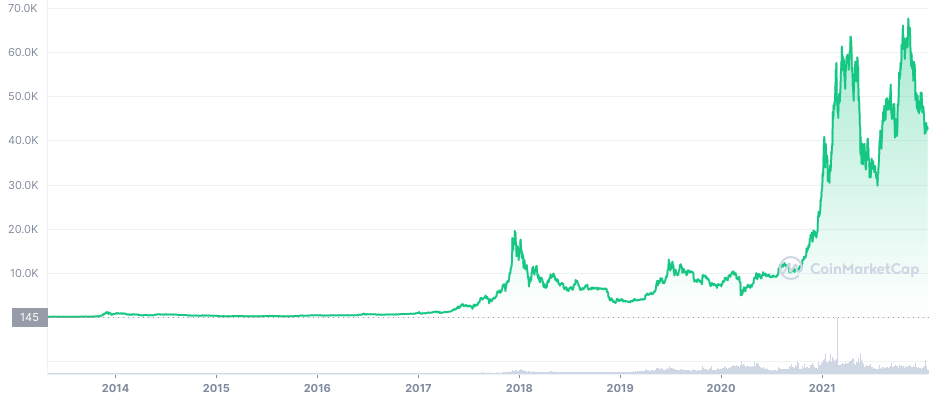
\includegraphics[width=\columnwidth]{figures/BTC_ALL_linear.png}
    \caption{Bitcoin linear price graph, attribution: CoinMarketCap \cite{coinmarketcap}}
    \label{btc-linear-figure}
\end{figure}

\begin{figure}[ht]
    \centering
    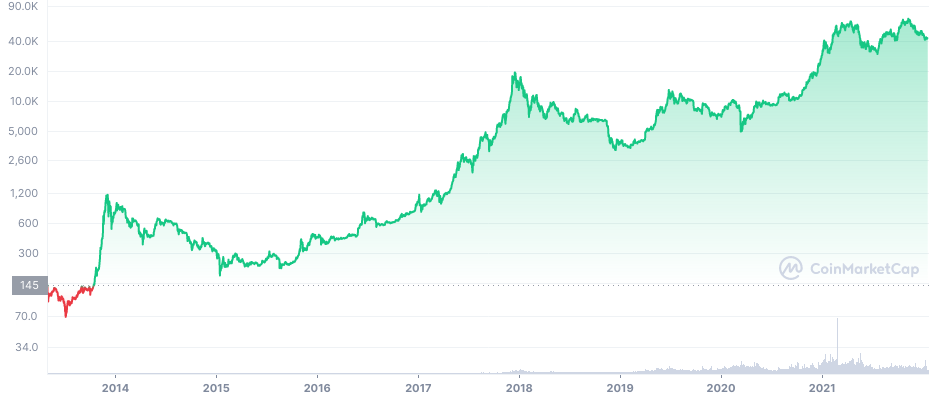
\includegraphics[width=\columnwidth]{figures/BTC_ALL_log.png}
    \caption{Bitcoin logarithmic price graph, attribution: CoinMarketCap \cite{coinmarketcap}}
    \label{btc-log-figure}
\end{figure}

\section{Data Analysis Provided by Supervisor}

The provided data were in the OHLCV \ref{ohlcv-candlestick-data} candlestick structure. A Python script converting these CSV data to a graph had to be created.

Data is analyzed in several ways:
\begin{enumerate}
    \item Correlation between coin's market price and its market capitalization.
    \item Correlation between coin's market price and the total market capitalization of the cryptocurrency market.
    \item Correlation between coin's market price and BTC price.
    \item Fundamental analysis of some bigger assets.
\end{enumerate}

\chapter{Adaptive Trading Strategy Proposals}
\label{proposal}


\section{Proposals}

Adaptive Trading Strategy Proposals:
\begin{enumerate}
    \item Risk metric
    \item Simple Moving Average crossover
    \item Machine Learning Series prediction
    \item {[BONUS]} Stablecoin shock peg/de-peg
\end{enumerate}

Variables to consider:
\begin{enumerate}
    \item strategies combinations
    \item adaptive vs classic model behavior ratio
    \item rebalance weights ratio and frequency
    \item different time intervals
    \item different size of coin portfolio

\end{enumerate}

Idea is to have e.g. 80\% of adaptive model behavior and 20\% of classic model behavior.

\section{Bull Market Behaviour}
During the possible Bull Market we hold coins, rebalance and buy more of them.

\section{Bear Market Behaviour}
During Bear Market we transfer our holding to stablecoins (in certain percentage) so that the market fall does not impede us.

\chapter{Adaptive Strategy Implementation}
\label{implementation}

\section{Framework or no framework}
During my search, I initially tinkered with several frameworks to test out their capabilities. The basic idea was that if a framework would prove satisfactory I would use it and tweak it to my needs so I do not reinvent the wheel again.

Alas, during my tinker with Python frameworks as backtrader, vectorbt or zipline, the frameworks were either outdated or they did not my needs of adaptive strategies.

\section{Trading data fetch}
Trading data that was used during the simluations were got from the supervisor. The data were not given at first, so I created a little script that got the data from Binance exchange. It was through their API and Python script that I could get historical data with any interval Binance supplied. That is also why I used this data when testing out shorter intervals than 1 day like 1 or 5 minutes.

\section{Testing out the Bitcoin Risk Metric}
\begin{enumerate}
    \item https://www.youtube.com/watch?v=ocQTqM4lL3k
    \item https://github.com/BitcoinRaven/Bitcoin-Risk-Metric-V2
\end{enumerate}

\chapter{Limitations and Further Improvements of Practical Deployment}
\label{limitations}

\chapter{Conclusion}
\label{conclusion}
